\section{Liverpool Life Meeting Records}
\label{sec.meeting_record}
As part of the APR requirements, each student, as a PhD candidate at Liverpool, must record the meeting times and content with their supervisor in a system called Liverpool Life. Below is a demonstration of how to operate it.

\begin{enumerate}
    \item First, go to the Liverpool Life website \url{https://liverpool-life.liverpool.ac.uk/} and log in with your Liverpool student number (not your email, and certainly not your XJTLU student number) and password.
    \item Find "PGR Record of Supervisory Meetings" and click "View all meetings".
    \item Click "Arrange new meeting"; a window will pop up where you enter the date and time, and select your supervisor (after you complete all the following steps, the selected supervisor will receive an email in their Liverpool inbox). Uncheck the first option "create calendar appointment"; otherwise, it will create an appointment in the Liverpool email calendar, which is mostly unused (because XJTLU students generally use the calendar system associated with their XJTLU email and probably never use the Liverpool calendar system). Then, check the option "has been pre-agreed" below.
    \begin{figure}[H]
        \centering
        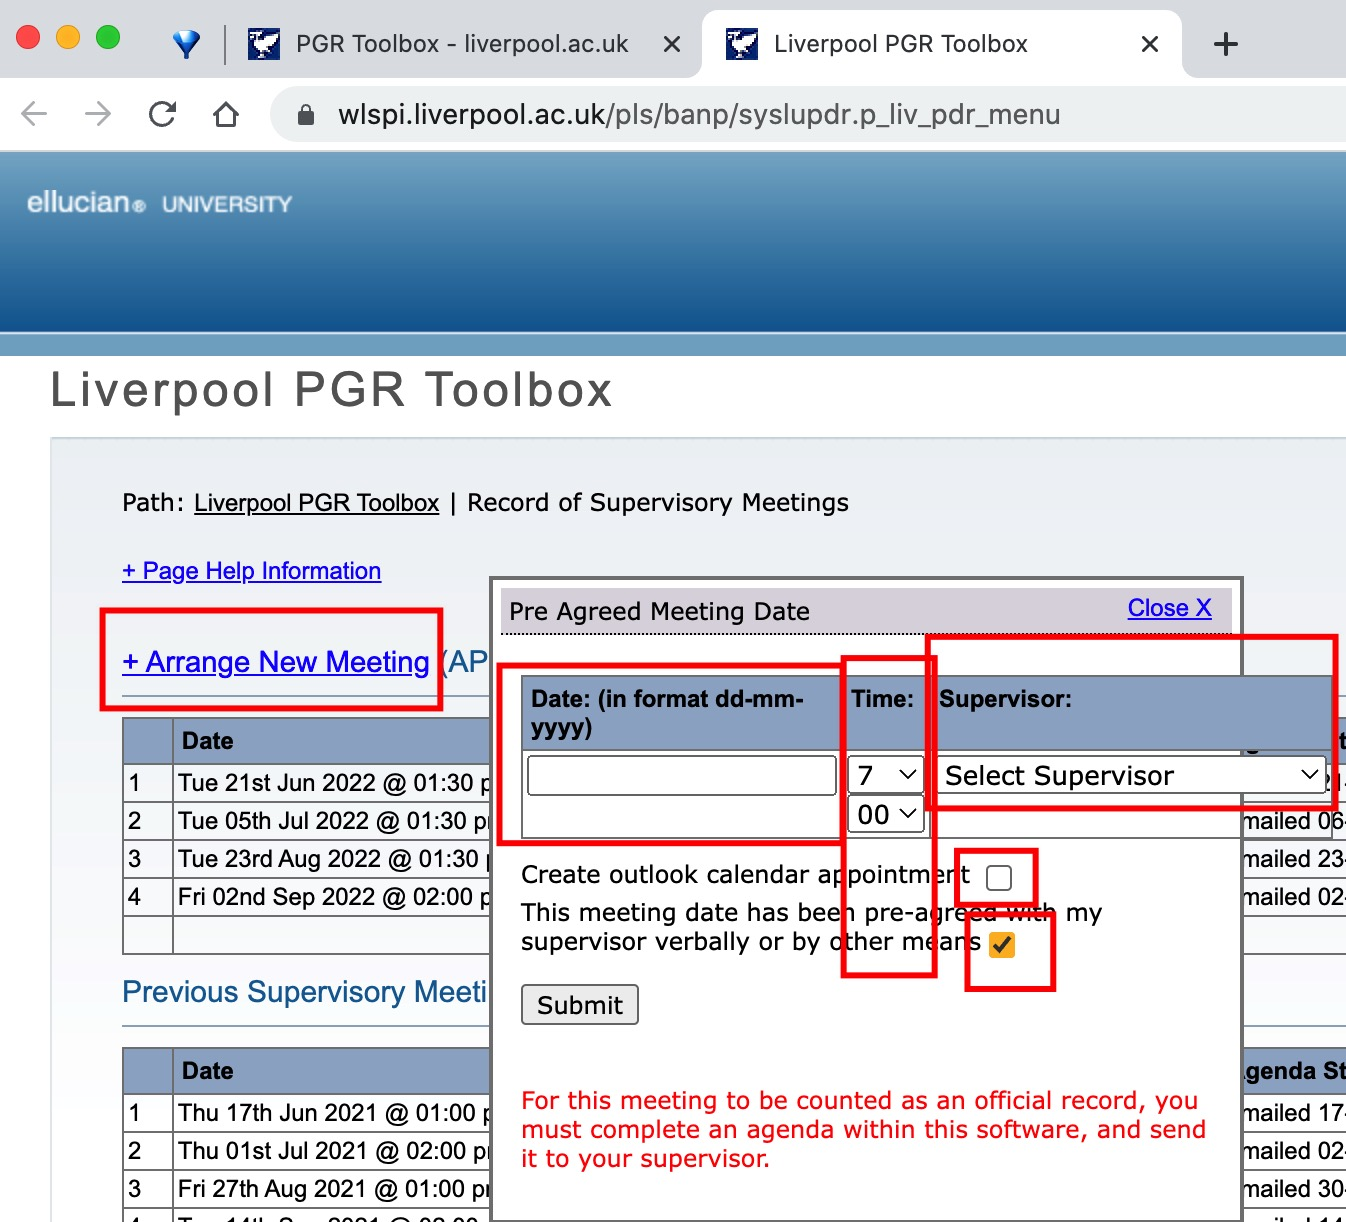
\includegraphics[width=0.5\columnwidth]{author-folder/Kai.Wu/meeting_record_figures/arange_new_meeting.jpg}
    \end{figure}
    \item Then recall what you discussed in your most recent meeting with your supervisor and fill in the progress report (what you have done), targets (what you plan to do before the next meeting), and discussion items.
    \begin{figure}[H]
        \centering
        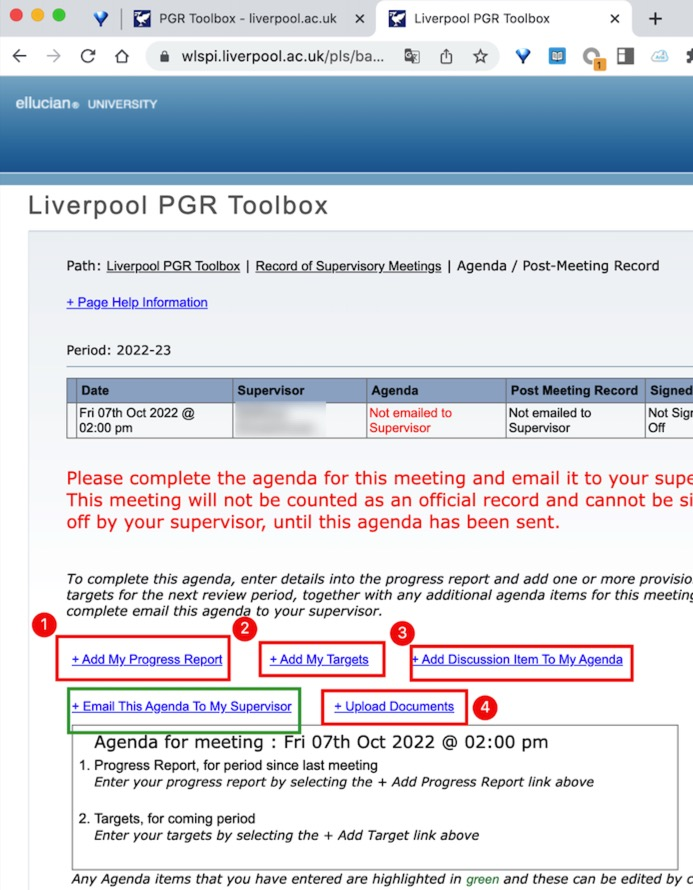
\includegraphics[width=0.5\columnwidth]{author-folder/Kai.Wu/meeting_record_figures/add_items_to_meetings.jpg}
    \end{figure}
    \item The content doesn't need to be extensive, but it shouldn't be too perfunctory either, as Liverpool will check it. After completing it, click "email this agenda", and both you and your supervisor will receive an automatically generated email in your Liverpool inboxes.
    \begin{figure}[H]
        \centering
        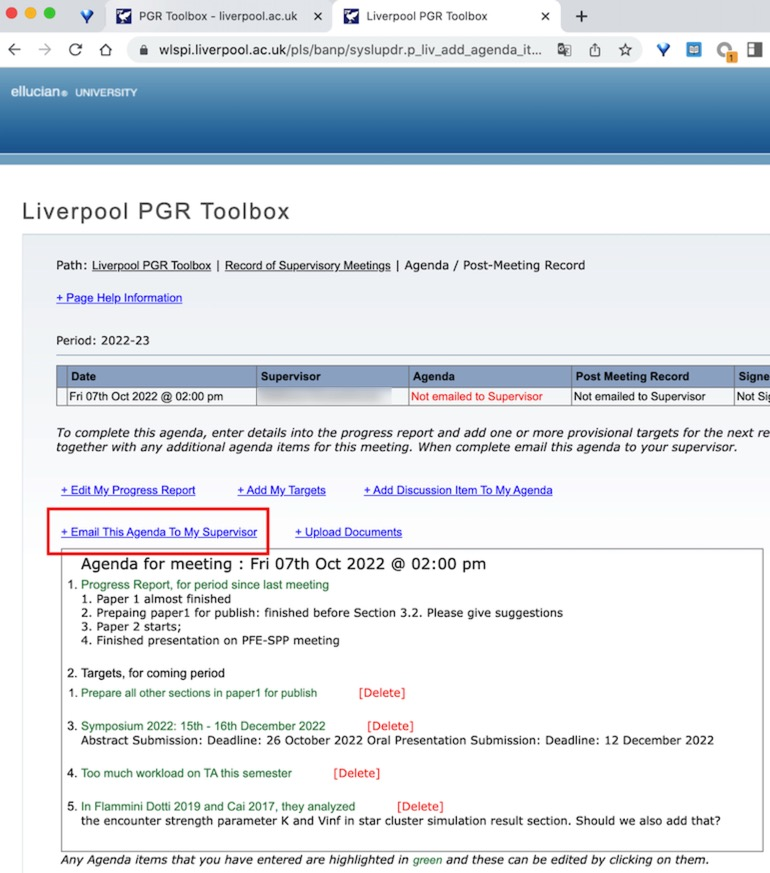
\includegraphics[width=0.5\columnwidth]{author-folder/Kai.Wu/meeting_record_figures/email_to.jpg}
    \end{figure}
    \item Don't be in a hurry to close it yet; you still need to fill in the comments from your meeting. Click "view edit meeting" on the right.
    \begin{figure}[H]
        \centering
        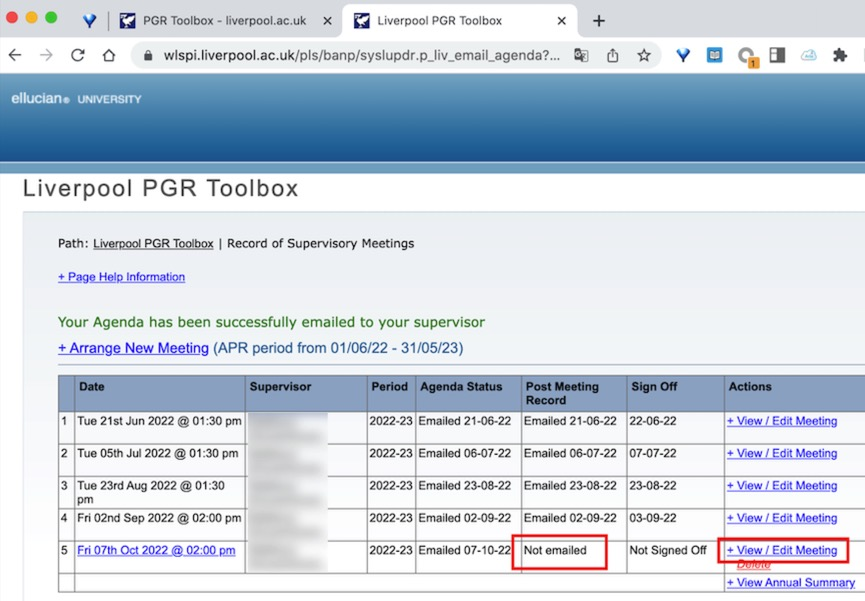
\includegraphics[width=0.5\columnwidth]{author-folder/Kai.Wu/meeting_record_figures/view_edit.jpg}
    \end{figure}
    \item Enter the comments from the meeting. Finally, click "email" at the top left, and you and your supervisor will receive another email in your Liverpool inboxes.
    \begin{figure}[H]
        \centering
        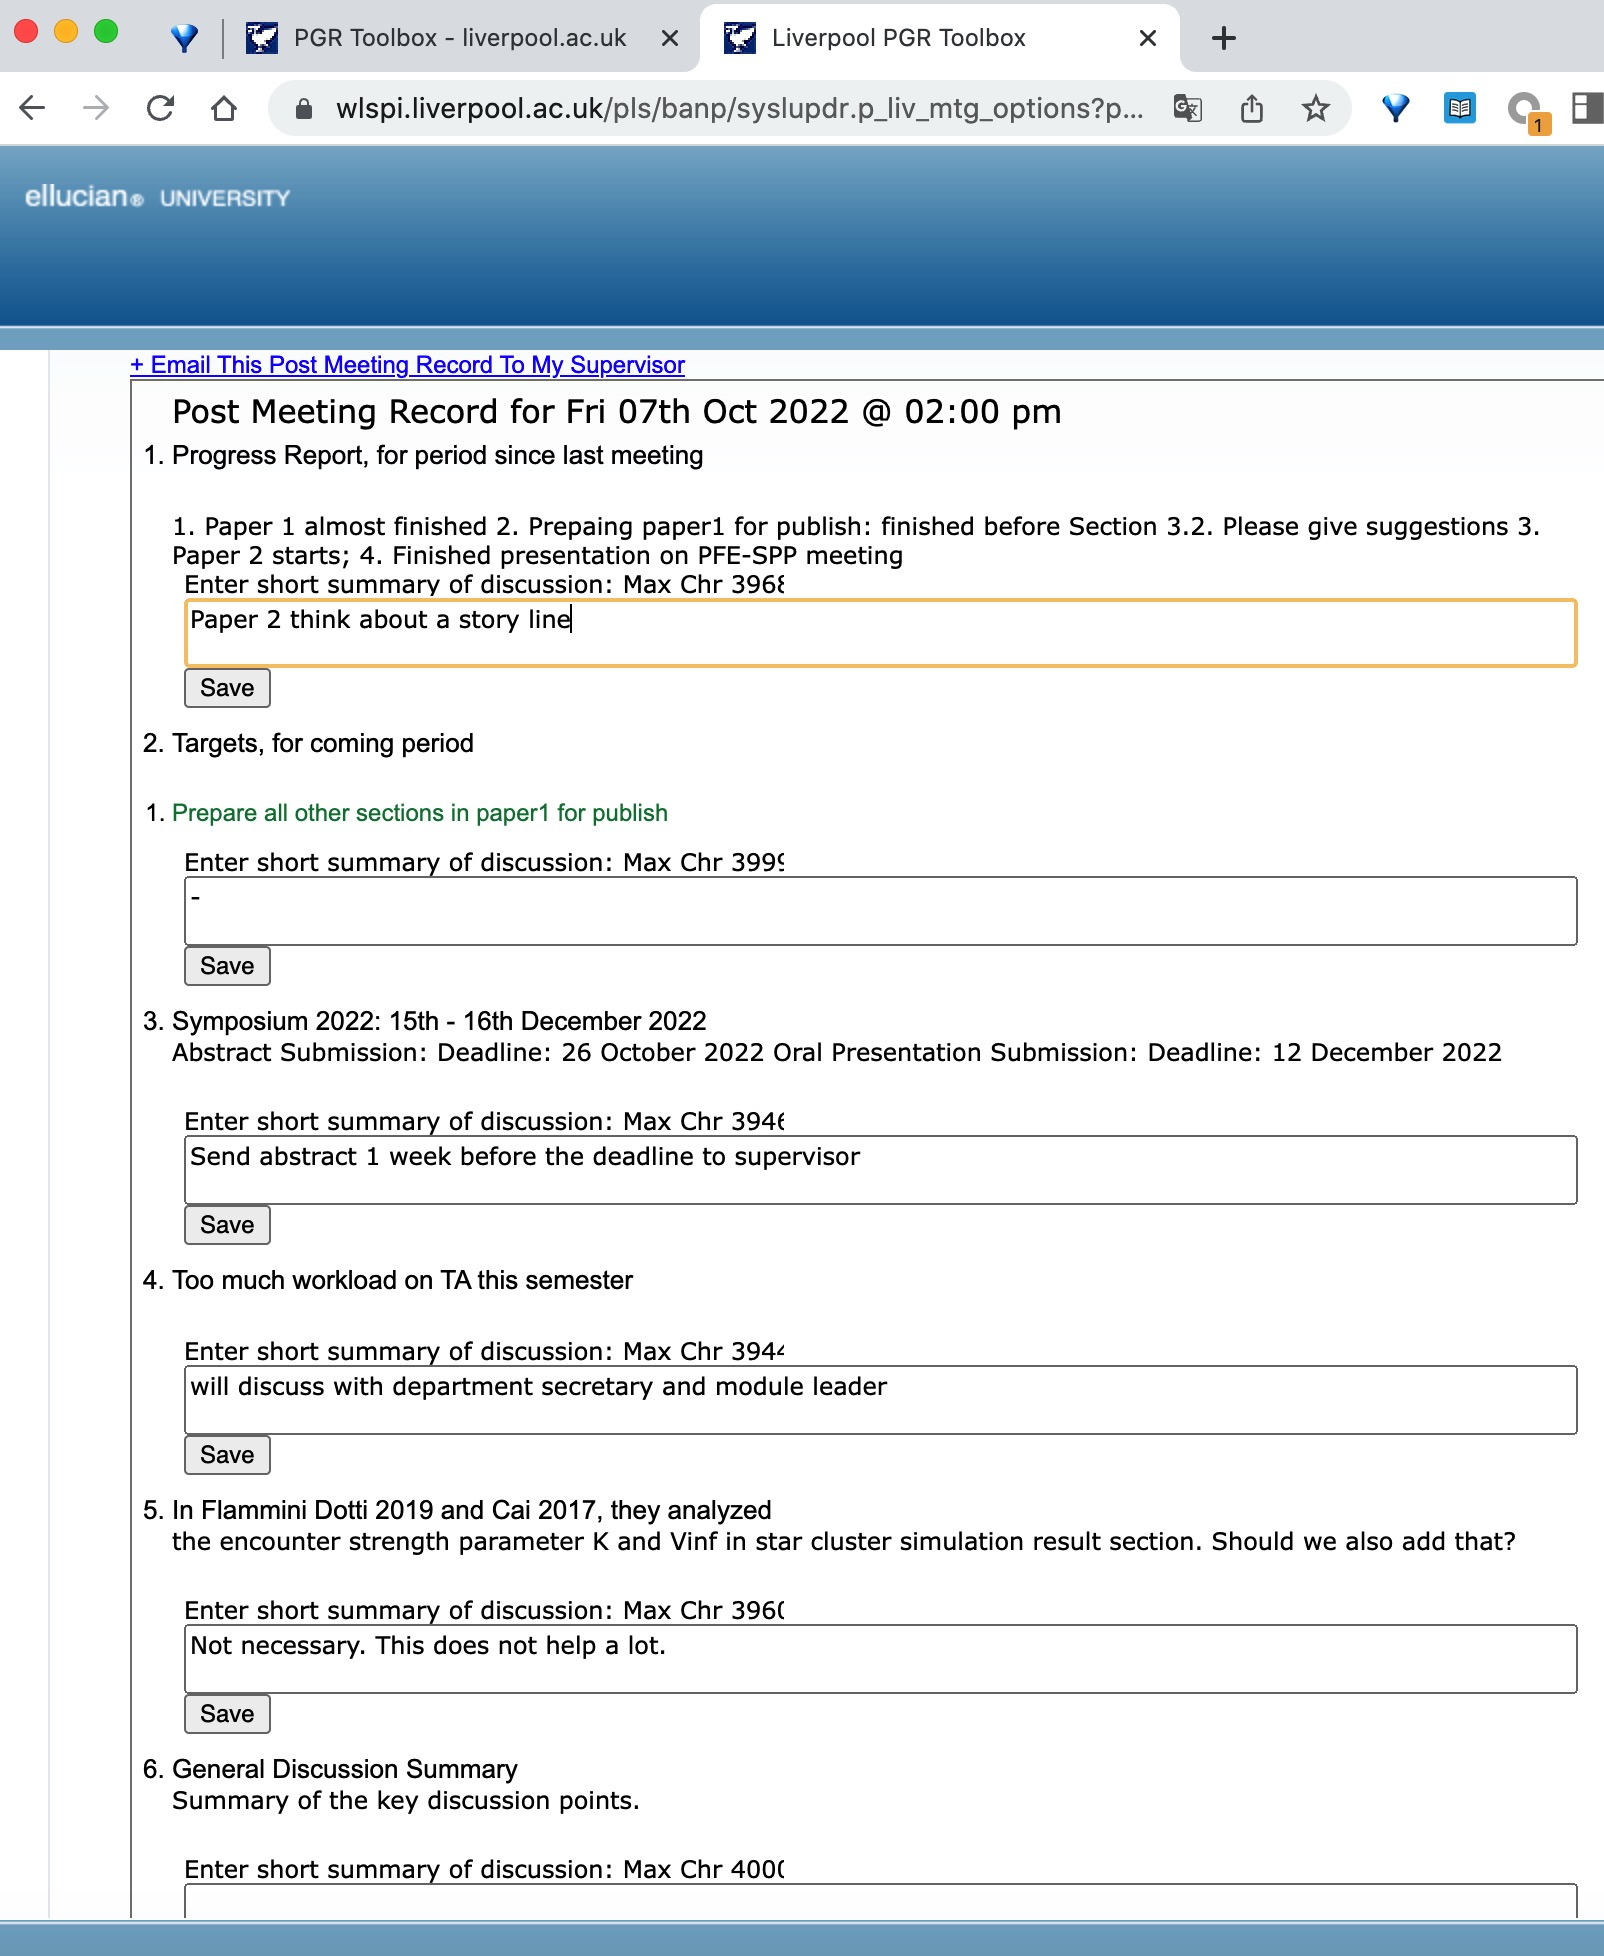
\includegraphics[width=0.5\columnwidth]{author-folder/Kai.Wu/meeting_record_figures/post_meeting.jpg}
    \end{figure}
    % \item 
    %     \begin{minipage}{0.3\textwidth}
    %         Due to the quirks of Liverpool Life, it is recommended to manually log out by clicking the top right corner in the Liverpool Life interface; otherwise, it may be difficult to log in next time.
    %     \end{minipage}
    %     \begin{minipage}{0.7\textwidth}
    %         \begin{figure}[H]
    %             \centering
    %             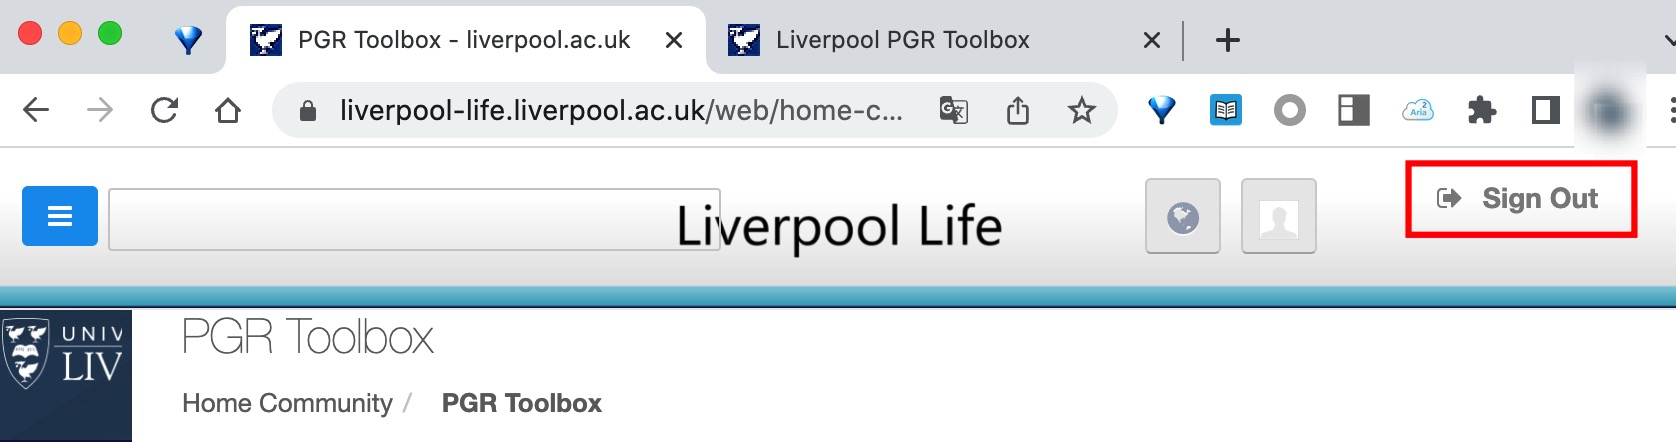
\includegraphics[width=0.9\columnwidth]{author-folder/Kai.Wu/meeting_record_figures/sign_out.jpg}
    %         \end{figure}
    %     \end{minipage}
    % \begin{figure}[H]
    %     \centering
    %     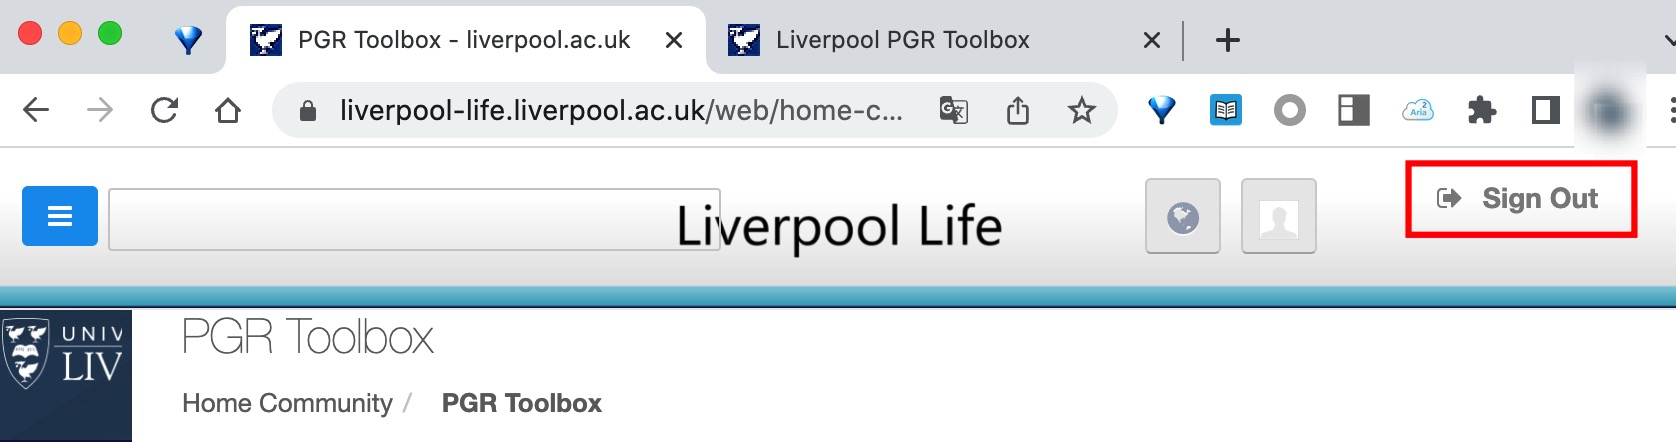
\includegraphics[width=0.5\columnwidth]{author-folder/Kai.Wu/meeting_record_figures/sign_out.jpg}
    % \end{figure}
    \item At this point, you're finished. Your supervisor needs to click "sign off" in the email they received in their Liverpool inbox. Afterwards, your Liverpool inbox will receive an email titled \textit{PGR Supervisor Meeting 5 (Fri 07th Oct 2022 @ 02:00 pm): sign off comments}, and this meeting record is then considered complete. Before each year's APR, all monthly meetings must be signed off at least once a month. If your supervisor hasn't signed off, you need to remind them.
\end{enumerate}

\vspace{5mm}
[Several Notes]
\begin{itemize}
    \item It's best to fill out this record once a month. Although you can make it up later—that is, not filling it out for several months and then filling in half a year's worth at once—is allowed, it's not standard practice. From my personal experience, if you wait until just before the APR to make it up, you'll either forget your progress over the year, or be too busy during the APR period. So, try to fill it out monthly as required.
    \item Liverpool Life and this reporting website often cannot be accessed! Due to various network and system issues, even using Wi-Fi and wired connections on the XJTLU campus, access is hit or miss. According to fellow students' experiences, using a VPN with a global proxy greatly improves connectivity, but such methods are not entirely legal and should not be taught to others, and absolutely should not be discussed on WeChat or QQ; otherwise, accounts may be blocked or groups may be banned. Students who cannot use VPNs should try to fill out the report early; otherwise, not being able to log in before the deadline will cause more anxiety.
\end{itemize}

\begin{flushright}
    (October 10, 2022 by \Wu) \\
    (Translated by GPT)
    \end{flushright}